 
% Para una visualizacion correcta, generar el PDF
% Ni el DVI ni el PS se visualizan bien

% Elegir el estilo que se desee, hay cientos en la red

\documentclass{beamer}
\usepackage{beamerthemeshadow}
\usepackage[galician]{babel}
\usepackage{eurosym}
% \usepackage[spanish]{babel}
\usepackage[utf8]{inputenc}
%\usepackage[latin1]{inputenc}

\begin{document}
\title[JDataMotion]{JDataMotion: unha ferramenta para a visualización dinámica de diagramas de dispersión}
\subtitle{Grao en Enxeñaría Informática \\
Universidade de Santiago de Compostela}  
\author{Autor: Pablo Pérez Romaní}
\institute
{
  \inst{}
  Director: Paulo Félix Lamas
  \and
  \inst{}
  Codirector: David González Márquez
}
\date{\today} 

\begin{frame}
\titlepage
\end{frame}

\frame{
\renewcommand{\baselinestretch}{0.75}\normalsize
\tableofcontents[hideallsubsections]
\renewcommand{\baselinestretch}{1.0}\normalsize
}

\section{Introdución} 

\begin{frame}
\frametitle{Introdución} 
Introdución
\end{frame}

\subsection{Introdución}
\begin{frame}
\frametitle{Introdución} 
\begin{itemize}
\item Na actual sociedade da información os datos crecen exponencialmente. Cobra valor a \textbf{minería de datos}, que ten por obxecto extraer deles \textbf{coñecemento} útil.
\item JDataMotion é unha solución a esta necesidade, que combina:
\vspace{-4mm}
\begin{itemize}
\item \textbf{Diagramas de dispersión}: axudan a atopar correlacións, distribucións ou tendencias entre os datos.
\item A noción de tempo como \textbf{compoñente dinámica} dos conxuntos de datos.
\end{itemize} 
\item O seu obxectivo é posibilitar a visualización e reprodución dos datos que se amosan sobre un diagrama de dispersión.
\end{itemize} 
\end{frame}

%%

\section{Xestión do proxecto} 

\begin{frame}
\frametitle{Xestión do proxecto} 
Xestión do proxecto
\end{frame}

\subsection{Metodoloxía de desenvolvemento}
\begin{frame}
\frametitle{Metodoloxía de desenvolvemento} 
\begin{itemize}
\item Premisas:
\begin{itemize}
\item Existencia de \textbf{riscos} de diversa gravidade.
\item Falta de experiencia na xestión de proxectos.
\item Proxecto aberto a cambios na especificación.
\item Necesidade de retroalimentación ao longo do desenvolvemento.
\end{itemize} 
\item Necesitamos unha metodoloxía áxil.
\item Escollemos metodoloxía \textbf{Scrum}.
\item Recorremos á ferramenta \textbf{Acunote} para xestionar os sprints e os requisitos funcionais asociados.
\item Elementos de configuración: código fonte e documentación. Xestionarémolos por medio da ferramenta \textbf{GitHub}.
\end{itemize} 
\end{frame}

%%

\section{Análise}
\begin{frame}
\frametitle{Análise} 
Análise
\end{frame}
\subsection{Requisitos}
\begin{frame}
\frametitle{Requisitos} 
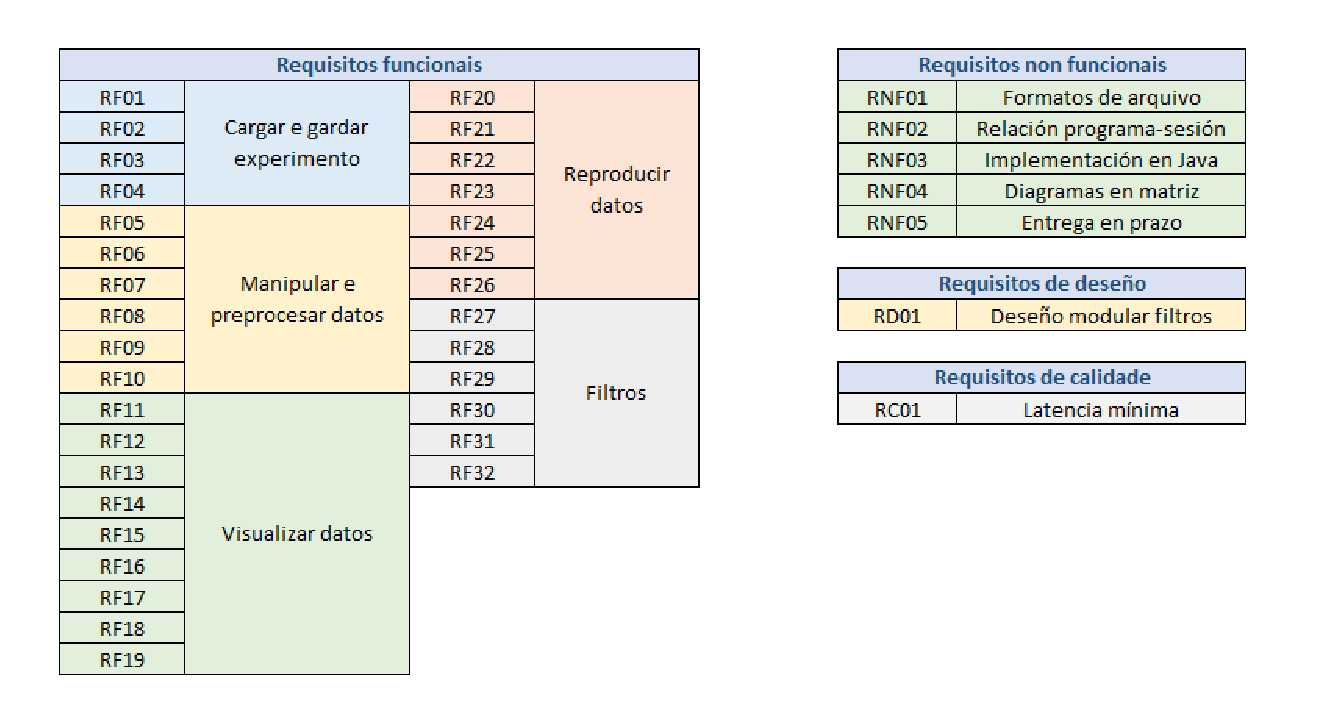
\includegraphics[width=\textwidth,height=\textheight,keepaspectratio]{figuras/docrequisitos}
\end{frame}

%%

\section{Deseño e implementación}
\begin{frame}
\frametitle{Deseño e implementación} 
Deseño e implementación
\end{frame}
\subsection{Deseño}
\begin{frame}
\frametitle{Deseño} 
\begin{itemize} 
\item O patrón \textbf{Modelo-Vista-Controlador} é a base da aplicación:
\begin{itemize} 
\item Modelo: almacena todos os datos cos que se traballa, xunto coa lóxica para manipulalos (filtros).
\item Vista: implementa a interface gráfica da aplicación.
\item Controlador: procesa en forma de comandos os eventos que a Vista recolle.
\end{itemize} 
\item O patrón \textbf{Observer} notifica á Vista calquera modificación no Modelo.
\item O patrón \textbf{Command} encapsula as transaccións (comandos) que poden modificar o Modelo.
\end{itemize} 
\end{frame}
\begin{frame}
\frametitle{Arquitectura} 
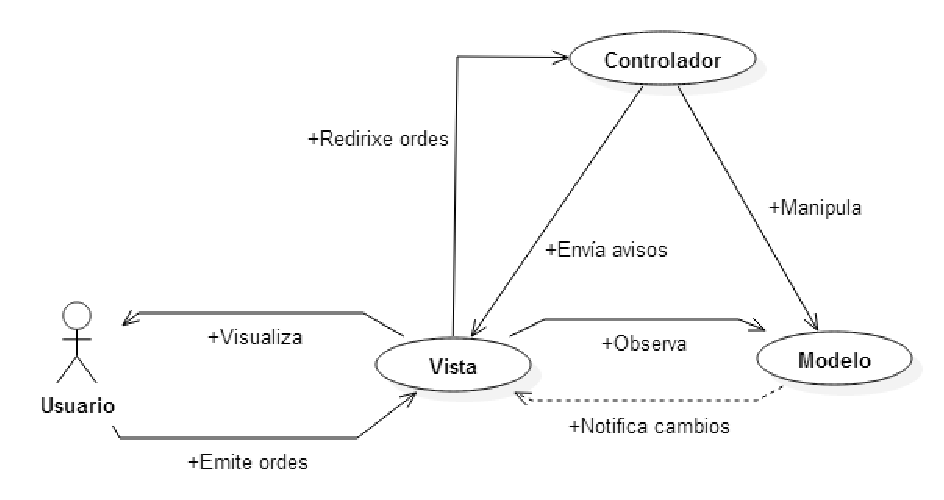
\includegraphics[width=\textwidth,height=\textheight,keepaspectratio]{figuras/MVC}
\end{frame}
\subsection{Modelo}
\begin{frame}
\frametitle{Modelo} 
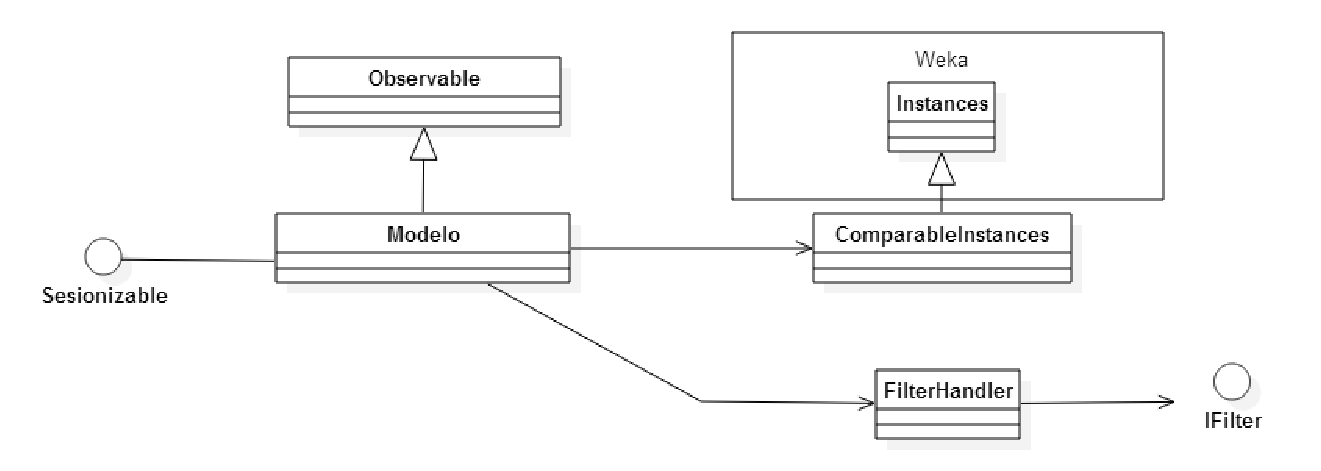
\includegraphics[width=\textwidth,height=\textheight,keepaspectratio]{figuras/modeloPresentacion}
\end{frame}
\subsection{Vista}
\begin{frame}
\frametitle{Vista} 
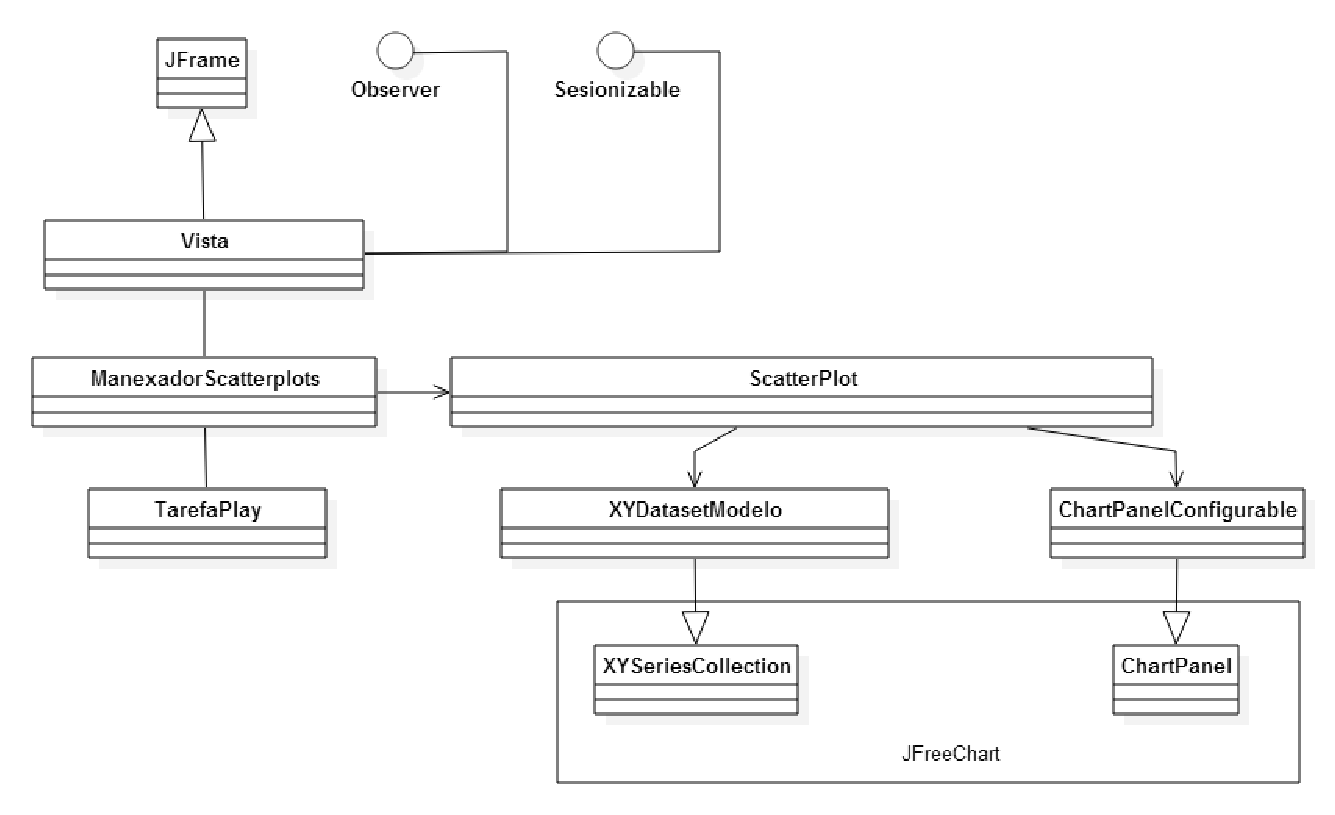
\includegraphics[width=\textwidth,height=\textheight,keepaspectratio]{figuras/vistaPresentacion}
\end{frame}
\subsection{Controlador}
\begin{frame}
\frametitle{Controlador} 
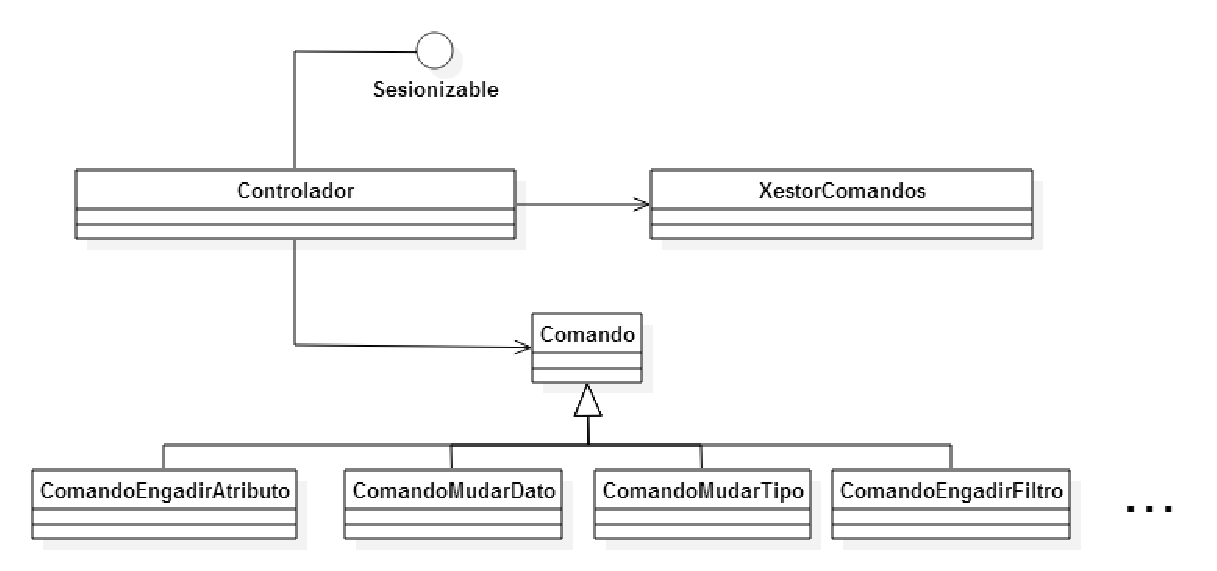
\includegraphics[width=\textwidth,height=\textheight,keepaspectratio]{figuras/controladorPresentacion}
\end{frame}

%%

\section{Validación e probas} 

\begin{frame}
\frametitle{Validación e probas} 
Validación e probas
\end{frame}

\subsection{Validación e probas}
\begin{frame}
\frametitle{Validación e probas} 
\begin{itemize} 
\item Dous métodos fundamentais de validación de requisitos:
\begin{itemize} 
\item \textbf{Tests de proba} (Instancias, atributos e filtros)
\item \textbf{Avaliación heurística} (Visualización)
\end{itemize} 
\item Para o \textbf{RC01} (latencia mínima), fíxose unha análise de prestacións. Mediuse latencia fronte a instancias e atributos, para a carga e a visualización dos datos.
\item Todos os tests validaron positivamente os requisitos que probaban.
\end{itemize} 
\end{frame}

\subsection{Análise de prestacións}
\begin{frame}
\frametitle{Análise de prestacións} 
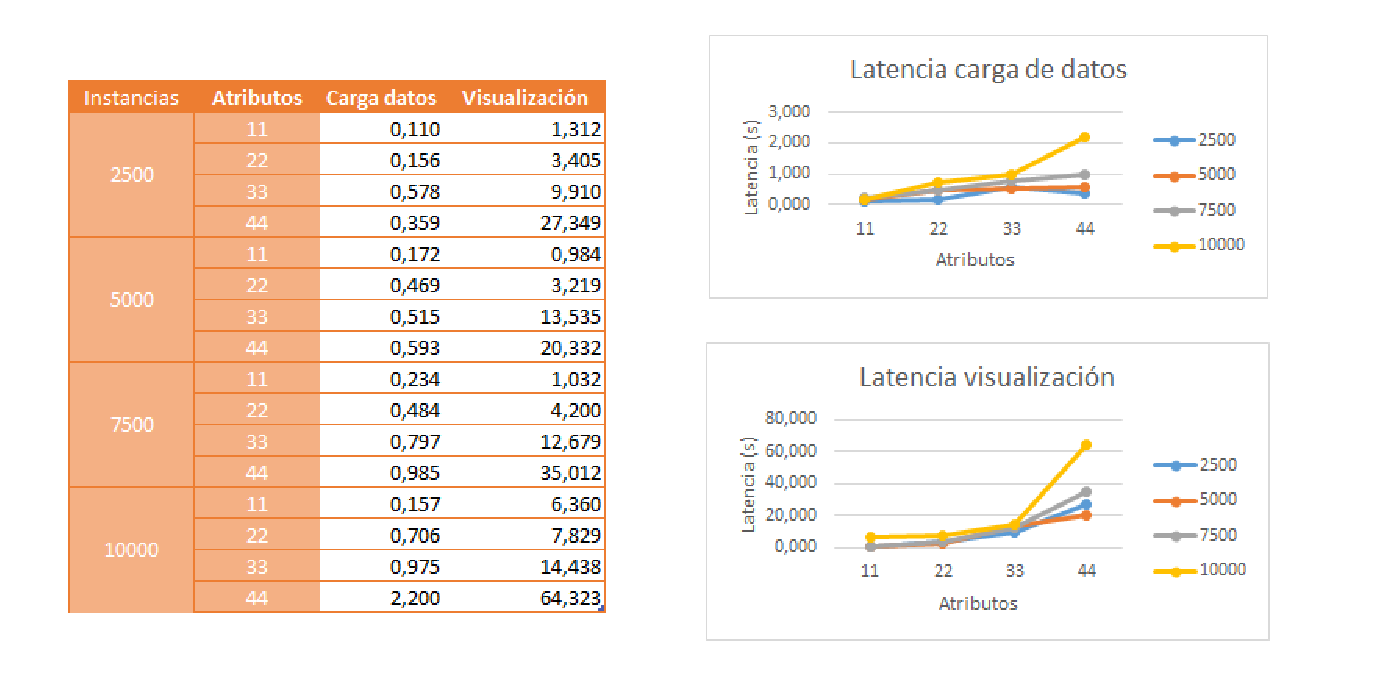
\includegraphics[width=\textwidth,height=\textheight,keepaspectratio]{figuras/eficiencia}
\end{frame}

%%

\section{Demo} 

\begin{frame}
\frametitle{Demo} 
Demo
\end{frame}

%%

\section{Conclusións} 

\begin{frame}
\frametitle{Conclusións} 
Conclusións
\end{frame}

\subsection{Conclusións}
\begin{frame}
\frametitle{Conclusións} 
\begin{itemize}
\item Aplicación de propósito xeral, que permite procesar e visualizar dinamicamente conxuntos de datos.
\item A metodoloxía Scrum facilitou a xestión de riscos e evitou que en certas fases nos afastásemos da especificación inicial.
\item Algunhas áreas de traballo propostas para un futuro desenvolvemento:
\begin{itemize}
\item Desvanecemento de puntos durante a reprodución.
\item Redución de latencia no proceso de visualización.
\item Migración de sesións.
\item Integración de plug-ins.
\item Asistente e/ou axuda.
\end{itemize}
\end{itemize} 
\end{frame}

\end{document}